\def\QRCODE{TB_IPR_TUT.IMG.shape_diagrams_pythonqrcode.png}
\def\QRPAGE{http://www.iptutorials.science/tree/master/TB_IPR/TUT.IMG.shape_diagrams/python}
\pcorrectionsection{Python correction}

\begin{python}
import numpy as np

import scipy.ndimage
import imageio # imread and imwrite
import matplotlib.pyplot as plt
import skimage.measure # some geometrical descriptors

# for reading files
import glob

from sklearn.cluster import KMeans
\end{python}

%
\subsection{Geometrical functionals}


The Crofton perimeter is defined by multiple projections, as well as the Feret diameter. Be careful while performing the rotation of the object (as it is a binary object, the interpolation method could introduce non integer values).

\begin{python}
def crofton_perimeter(I):
    """ Computation of crofton perimeter
    """
    inter = [];
    h = np.array([[1, -1]]);
    for i in range(4):
        II = np.copy(I);
        I2 = scipy.misc.imrotate(II, 45*i,interp='nearest');
        I3 = scipy.ndimage.convolve(I2, h);
        
        inter.append(np.sum(I3>100));
        
        
    crofton = np.pi/4. * (inter[0]+inter[2] + (inter[1]+inter[3])/np.sqrt(2));
    return crofton

\end{python}

\begin{python}
def feret_diameter(I):
    """ 
    Computation of the Feret diameter
    minimum: d (meso-diameter)
    maximum: D (exo-diameter)
    
    Input: I binary image
    """
    d = np.max(I.shape);
    D = 0;
    
    for a in np.arange(0, 180, 30):
        I2 = scipy.misc.imrotate(I, a, interp='nearest');
        F = np.max(I2, axis=0);
        measure = np.sum(F>100);
        
        if (measure<d):
            d = measure;
        if (measure>D):
            D = measure;
    return d,D;
\end{python}

The inscribed circle is just the maximum of the distance transform inside the object. The distance map for an image apple is shown in Fig.\ref{fig:shape_diagrams:python:shapes:dm}.
\begin{python}
def inscribedRadius(I):
    """
    computes the radius of the inscribed circle
    """
    dm = scipy.ndimage.morphology.distance_transform_cdt(I>100);
    radius = np.max(dm);
    return radius;
\end{python}

\begin{figure}[H]
\centering\caption{Illustration of the computation of two shape parameters.}
\subfloat[Distance map of an object apple. The inverse is actually displayed in order to see correctly the progression. The maximum of the distance map is the radius of the inscribed circle.]{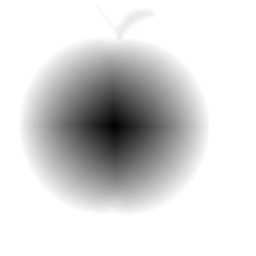
\includegraphics[width=.45\linewidth]{distancemap.png}\label{fig:shape_diagrams:python:shapes:dm}}
\hfill
\subfloat[Circumscribed circle.]{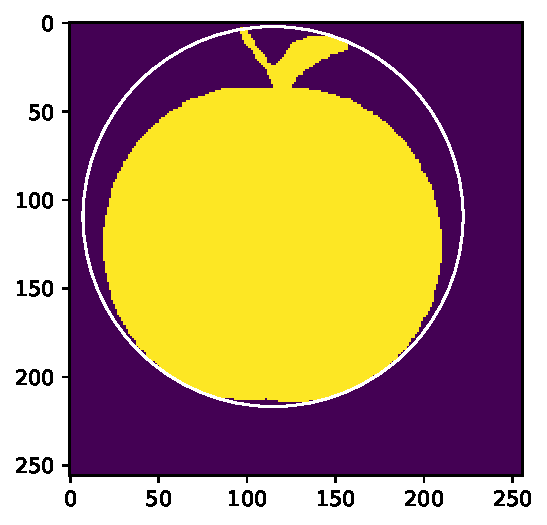
\includegraphics[width=.45\linewidth]{circum.pdf}\label{fig:shape_diagrams:python:shapes:circum}}%
\label{fig:shape_diagrams:python:shapes}%
\end{figure}

The smallest enclosing circle is computed by using the code from the Project Nayuki\footnote{https://www.nayuki.io/page/smallest-enclosing-circle} published under the GNU Lesser General Public License. The result is presented in Fig.\ref{fig:shape_diagrams:python:shapes:circum}.
\begin{python}
def circumCircle(I):
    """
    this version uses a function provided by Project Nayuki
    under GNU Lesser General Public License
    """
    points = np.argwhere(I > 100);
    c = smallestenclosingcircle.make_circle(points);
    return c;
\end{python}

\subsection{Shape diagrams}
The shape diagrams are constructed by reading all the images and computing the shape descriptors.
\begin{python}
def diagrams():
    name=['apple-*.bmp', 'Bone-*.bmp', 'camel-*.bmp'];
    elongation=[];
    thinness=[];
    roundness=[];
    z=[];
    for pattern in name:
        namesList = glob.glob(pattern);
        for fichier in namesList:
            I = imageio.imread(fichier);
            radius = inscribedRadius(I);
            d,D = feret_diameter(I);
            crofton = crofton_perimeter(I);
            
            elongation.append(d/D);
            thinness.append(2*radius / D);
            roundness.append(4*np.sum(I>100)/(np.pi * D**2));
            z.append(crofton / (np.pi * D));
\end{python}
    
The display of the different plots is just a use of the function \pinline{plt.plot}.
\begin{python}
    plt.plot(elongation[0:20], thinness[0:20], "o", label='Apple')
    plt.plot(elongation[20:40], thinness[20:40], "+", label='Bone')
    plt.plot(elongation[40:60], thinness[40:60], ".", label='Camel')
    plt.legend(name)
    plt.show
    evaluateQuality(elongation, thinness);
    
    plt.figure();
    plt.plot(z[0:20], roundness[0:20], "o", label='Apple')
    plt.plot(z[20:40], roundness[20:40], "+", label='Bone')
    plt.plot(z[40:60], roundness[40:60], ".", label='Camel')
    plt.legend(name)
    plt.show
    evaluateQuality(z, roundness);
    
    plt.figure();
    plt.plot(thinness[0:20], z[0:20], "o", label='Apple')
    plt.plot(thinness[20:40], z[20:40], "+", label='Bone')
    plt.plot(thinness[40:60], z[40:60], ".", label='Camel')
    plt.legend(name)
    plt.show
    evaluateQuality(thinness, z);
\end{python}

\vspace*{-10pt}

\subsection{Shape classification}

The following code evaluates the quality by comparing the known class of the shape with the segmented (via the kmeans method) class. The result is illustrated in Fig.\ref{fig:shape_diagrams:python:kmeans} with an accurary of 98.3\%.

\begin{python}
def evaluateQuality(x, y):
    global i
    n = 3;
    k_means = KMeans(init='k-means++', n_clusters=n)
    X = np.asarray(x);
    Y = np.asarray(y);
    pts = np.stack((X, Y));
    pts = pts.T;
    #print(pts)
    k_means.fit(pts);
    k_means_labels = k_means.labels_;
    k_means_cluster_centers = k_means.cluster_centers_;
    # plot
    fig = plt.figure()
    colors = ['#4EACC5', '#FF9C34', '#4E9A06']
    # KMeans
    for k, col in zip(range(n), colors):
        my_members = k_means_labels == k
        cluster_center = k_means_cluster_centers[k]
        plt.plot(pts[my_members, 0], pts[my_members, 1], 'o',
                markerfacecolor=col,  markersize=6)
        plt.plot(cluster_center[0], cluster_center[1], 'o', markerfacecolor=col,
                markeredgecolor='k', markersize=12)
    plt.title('KMeans')
    plt.show()
    fig.savefig("kmeans"+str(i)+".pdf");
    i += 1;
    """
    Evaluation of the quality: count the number of shapes correctly detected
    """
    accuracy = np.sum(k_means_labels[0:20]  == scipy.stats.mode(k_means_labels[0:20]));
    accuracy +=np.sum(k_means_labels[20:40] == scipy.stats.mode(k_means_labels[20:40]));
    accuracy +=np.sum(k_means_labels[40:60] == scipy.stats.mode(k_means_labels[40:60])); 
    accuracy = accuracy / 60 * 100;
    print('Accuracy: {0:.2f}%'.format(accuracy));
\end{python}

\begin{figure}[H]
\centering
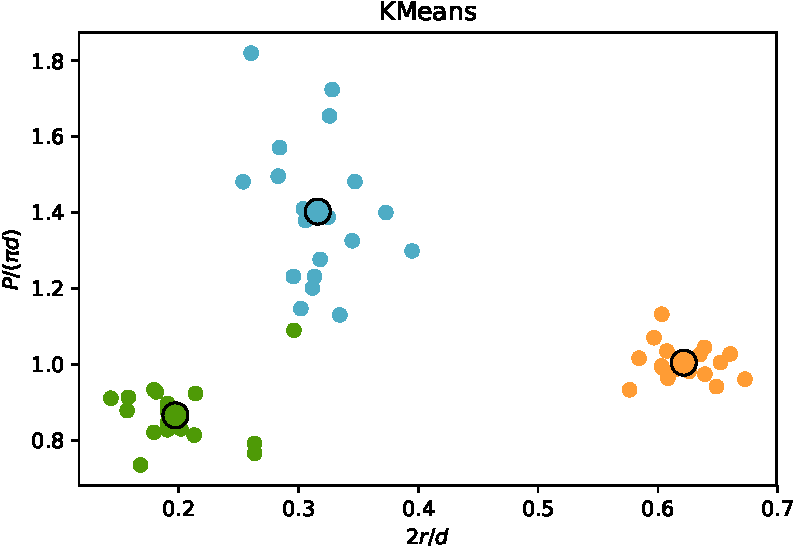
\includegraphics[width=0.8\textwidth]{kmeans2-crop.pdf}
\caption{\textls[-22]{Illustration of the accuracy of the classification from a k-means method. The k-means method is not necessarily the adapted to these data. The measured accurary if of 98.3\%.}}
\label{fig:shape_diagrams:python:kmeans}

\end{figure}
